\documentclass[sigconf,anonymous,nonacm]{acmart}
\settopmatter{printacmref=false}
\setcopyright{none}
\acmConference[RAIOps4Fin 2026]{Workshop on Applied Responsible AI Operations for Finance}{November 14, 2026}{Milan, Italy}
\acmYear{2026}
\title{Fail-Closed Point-in-Time Ledger Audits for Financial AI Evaluation}
\subtitle{Author-review draft; not submitted}
\author{Anonymous Authors}
\renewcommand{\shortauthors}{Anonymous Authors}
\begin{document}
\begin{abstract}
A financial evaluation can report plausible returns even when its features or training labels were unavailable at the decision time. We present a small, dependency-free ledger audit that makes this inconsistency a publication-blocking failure. The input contract records decision time, latest feature availability, latest training-label availability, target end, target exposure and asset return for each interval. Only a fully valid ledger produces hypothetical strategy and matched baseline paths; otherwise every performance field is withheld. We evaluate the implementation with a fixed enumeration of 58 synthetic controls derived from one retained six-interval ledger. All 55 invalid controls are rejected, while the original ledger and two equivalent timezone representations pass with identical metrics. Fifteen independent Decimal-oracle comparisons across five declared transaction-cost settings agree with binary-floating-point results within $3.44\times10^{-16}$ absolute total-return error. The retained valid strategy loses 2.446481\%, illustrating that an integrity pass is not a favorable economic finding. The contribution is an executable evaluation control and a transparent failure corpus, not a trading strategy, independent timestamp certification, or evidence of production adoption.
\end{abstract}
\keywords{financial AI evaluation, point-in-time integrity, reproducibility, auditability, synthetic controls}
\maketitle

\section{Introduction}
Financial AI evaluation connects several different objects: a predictive model, the information available when a decision was made, a sequence of exposures, and an accounting rule. A final return number does not disclose whether these objects are mutually consistent. A model can use a future-released feature while its return arithmetic remains perfectly reproducible. Conversely, a correctly timed ledger can describe an unprofitable strategy. Operational review needs to keep these questions separate.

Leakage has been documented as a recurring cause of overoptimistic machine-learning findings. Kapoor and Narayanan provide a taxonomy and advocate explicit model information sheets~\cite{kapoor2023}. Reproducibility programs also emphasize accessible code, data and reporting practices~\cite{pineau2021}. Our narrower question is operational: can a frozen, single-asset prediction ledger enforce a declared information-time contract before exposing any performance number?

We implement this question as a fail-closed software control. An accepted input produces interval-level hypothetical returns for three paths under one explicit cost rule. An invalid input produces row-level findings and no performance paths, including baselines. This makes a validation failure part of the report schema rather than a warning that can be detached from a favorable headline.

The contribution has three parts. First, a small input contract distinguishes decision, availability and target times. Second, reproducible fault-location controls test both rejection and the preservation of equivalent timestamp spellings. Third, an independent decimal calculation checks the cost arithmetic without calling the implementation's return function. These contributions are bounded to software behavior. No observed market dataset, fitting procedure, new forecasting experiment, or deployment study is introduced.

\section{Scope and Input Contract}
\subsection{One row, one decision interval}
Each row contains exactly six named fields. For row $i$, let $t_i$ be the decision instant, $a_i$ the latest availability instant across all features used, $\ell_i$ the latest availability instant across training labels used, and $u_i$ the target interval end. Let $p_i$ be the declared target exposure and $r_i$ the simple asset return over the corresponding interval. All time fields must include a UTC offset and are compared after conversion to UTC.

The accepted contract is
\begin{align}
 a_i &\leq t_i, &\ell_i &\leq t_i, &u_i &> t_i,\\
 t_{i+1} &> t_i, &t_{i+1} &= u_i, &-1&\leq p_i\leq 1.
\end{align}
The second equality requires contiguous, non-overlapping intervals. It prevents the report from quietly skipping an unobserved interval or compounding overlapping returns. Returns must be finite and strictly greater than $-1$. The schema also rejects missing or duplicate columns, inconsistent row width, empty data, nonfinite exposures and naive timestamps.

These are deliberately restrictive semantics. The tool is not a multi-asset portfolio simulator and does not support asynchronous assets, leverage above unit exposure, missing intervals, changing universes or zero-wealth paths. A workflow requiring these features needs an explicit alternative contract, rather than an exception that silently weakens this one.

\subsection{Assertions and their evidence}
The availability fields are assertions from the ledger producer. Checking $a_i\leq t_i$ does not establish that $a_i$ is the actual release time of a market observation. The ledger can still be misleading if the producer supplies false timestamps, omits a used feature, reports a training cutoff incorrectly, or computes returns from an inappropriate price series. No internal arithmetic check resolves those questions.

The configuration therefore requires a nonempty source description, asset label, license description, protocol identifier and invalidation condition, as well as an explicit synthetic/observed designation and numerical fee and slippage assumptions. The tool hashes the exact CSV bytes it consumes and a canonical serialization of the configuration. These hashes identify the audited objects; they do not certify their truth, permission status or financial suitability.

\section{Fail-Closed Evaluation}
\subsection{Report generation}
The implementation first records findings about schema, parsing, time ordering, availability, intervals and numeric values. Each check exposes its identifier, status, number of findings and a bounded list of affected CSV rows. It preserves the consumed-byte digest even if the ledger fails. Performance calculation is entered only after all input checks pass.

If a return path would leave finite positive arithmetic, the report becomes a failure and all performance paths are withheld. This includes a valid-looking strategy paired with an unsupported baseline. Downstream consumers can require both an overall pass and non-null performance, rather than independently interpreting a collection of warning strings. The command-line workflow refuses an existing output path so a failed or revised run cannot overwrite an earlier retained artifact.

\subsection{Declared transaction-cost approximation}
The arithmetic uses an exposure-change approximation, not an execution simulator. For combined one-way cost $c=(f+s)/10^4$, where $f$ and $s$ are fee and slippage basis points, define
\begin{align}
 q_i &= |p_i-p_{i-1}|+\mathbf{1}_{i=n}|p_i|,\quad p_0=0,\\
 g_i &= p_i r_i-cq_i,\qquad W_i=W_{i-1}(1+g_i),\quad W_0=1.
\end{align}
The final term charges terminal liquidation. A direct reversal from $-1$ to $+1$ trades two units of target exposure. The report exposes the period exposure changes, costs, gross returns, net returns and wealth path in addition to total return and maximum drawdown.

Buy-and-hold applies unit exposure over the same intervals and pays opening and closing costs. Cash holds zero exposure and earns zero interest. These baselines share the same accounting approximation and audited interval sequence. The implementation does not simulate drift-induced rebalancing, financing, securities lending, impact, execution prices, taxes or corporate actions. Consequently, even valid observed inputs would produce hypothetical ledger arithmetic, not verified realized returns.

\begin{table}[t]
\caption{The retained arithmetic fixture. Positions and asset returns were manually specified. They are not market observations.}
\label{tab:ledger}
\centering
\begin{tabular}{rrrr}
\toprule
Interval & Exposure & Asset return (\%) & Traded units\\
\midrule
1 & $1$ & $1.0$ & $1$\\
2 & $-1$ & $1.5$ & $2$\\
3 & $0$ & $-2.0$ & $1$\\
4 & $0.5$ & $0.5$ & $0.5$\\
5 & $-0.5$ & $1.2$ & $1$\\
6 & $1$ & $-0.8$ & $2.5$\\
\bottomrule
\end{tabular}
\end{table}

\section{Control Study}
\subsection{Fixed enumeration}
The study starts from the retained six-interval synthetic ledger in Table~\ref{tab:ledger}. Its byte digest is checked before analysis, so a substituted input cannot silently become the same study. No prices, model predictions or outcome-bearing research splits are fetched.

The enumeration contains three valid controls: the original representation and two equivalent spellings of every timestamp using UTC offsets of $-07{:}00$ and $+05{:}30$. The expected result is an identical performance object for all three, because the instants have not changed.

For each of six row locations, the study independently introduces a one-second future feature, one-second future training label, zero-length target interval, exposure of $1.01$, nonfinite return, or naive decision timestamp. For each of the five internal boundaries it independently introduces a one-second gap, one-second overlap, or duplicate decision. Four additional cases exercise an empty ledger, a missing column, an extra column and a duplicate header. Each mutant begins from the original input; errors do not accumulate across cases. The resulting 55 invalid controls test specified contract violations, not naturally occurring failure prevalence.

The success criterion is strict. Each invalid control must fail overall, record the expected check identifier and expose no performance. Each valid control must pass all checks and retain the original performance object. The script writes every mutated CSV, every complete report and a digest manifest, allowing a reviewer to inspect the exact fault rather than rely on a summarized test count.

\subsection{Independent arithmetic oracle}
A second calculation uses Python Decimal at 70-digit precision and parses numeric values directly from the retained CSV strings. It does not call the implementation's return routine. It independently accumulates exposure changes, terminal liquidation, net period returns and compounded wealth for strategy, buy-and-hold and cash at combined one-way costs of 0, 1, 5, 10 and 25 basis points.

The grid is an arithmetic stress check. Its values are not fitted, selected or promoted on the basis of economic performance. The predetermined acceptance tolerance is $10^{-14}$ absolute total-return difference, with exact turnover agreement and $10^{-15}$ absolute period-return tolerance. No sampling distribution, statistical significance claim or confidence interval is attached to these deterministic comparisons.

\begin{table}[t]
\caption{All 58 controls matched their expected classifications. Each listed invalid case withheld all performance fields. Counts enumerate locations in one synthetic fixture.}
\label{tab:controls}
\centering
\begin{tabular}{lrr}
\toprule
Family & Cases & Expected result\\
\midrule
Original and equivalent offsets & 3 & Pass\\
Future feature availability & 6 & Fail\\
Future training-label availability & 6 & Fail\\
Zero-length target interval & 6 & Fail\\
Unsupported exposure & 6 & Fail\\
Nonfinite asset return & 6 & Fail\\
Naive decision timestamp & 6 & Fail\\
Gap / overlap / duplicate decision & 15 & Fail\\
Schema or empty-data faults & 4 & Fail\\
\bottomrule
\end{tabular}
\end{table}

\section{Results}
All 58 classifications match the expected outcomes (Table~\ref{tab:controls}). The three valid controls return identical performance objects. All 55 invalid controls withhold the strategy and both baseline paths. In particular, moving the latest feature or training-label availability one second beyond the decision is detected at every row location. This establishes the behavior on those controlled errors; it does not estimate sensitivity to falsified metadata or an unknown distribution of operational defects.

The 15 Decimal comparisons agree within a maximum absolute total-return discrepancy of $3.44\times10^{-16}$, below the specified tolerance. Turnover matches exactly. At the original 5-basis-point fee plus 5-basis-point slippage setting, the hypothetical strategy return is $-2.446481\%$, buy-and-hold is $+1.158764\%$, and cash is $0\%$. Strategy turnover is 8 exposure units, compared with 2 for buy-and-hold. The strategy's period cost fractions sum to $0.008$; this sum is not itself a compounded return difference.

\begin{figure}[t]
\centering
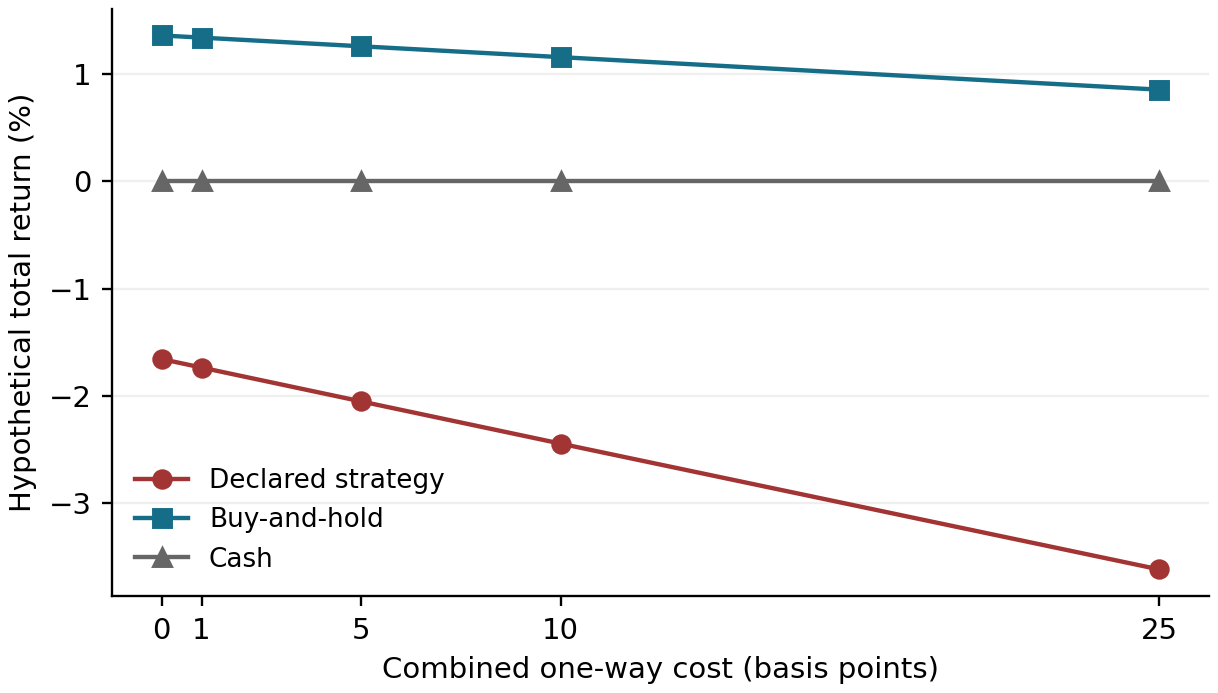
\includegraphics[width=\linewidth]{figures/cost_arithmetic.png}
\Description{Three hypothetical return curves evaluated at combined one-way costs of 0, 1, 5, 10 and 25 basis points. Strategy returns are negative throughout, buy-and-hold returns are positive and decrease with costs, and cash remains zero.}
\caption{Independent Decimal arithmetic for the same retained synthetic exposure sequence across five fixed combined one-way cost settings. The sweep tests the cost calculation; it is not model selection or market performance.}
\label{fig:cost}
\end{figure}

An integrity pass therefore cannot be interpreted as strategy quality. The deliberately losing valid control is useful precisely because it separates input consistency from economic desirability. Conversely, the future-feature twin keeps exposures and asset returns unchanged while invalidating the information contract. A return-only calculation would be numerically unchanged even though publication of that performance is blocked by the full audit.

The pre-existing OHLCV fixture corpus remains a separate regression check: its 70 expected classifications and retained summary are unchanged. It checks a different input layer and is not added to the 58-ledger denominator. Likewise, previously closed forecasting studies are neither rerun nor included as evidence that this audit improves prediction. The control study evaluates software behavior, not predictive efficacy.

\section{Operational Use and Reproduction}
The intended insertion point is after a research workflow freezes a ledger and before a report publishes performance. A producer exports rows under the contract. The audit consumes one byte snapshot, emits a machine-readable report and retains either validated paths or explicit findings. A reviewer can then compare the declared source and timing metadata with independent release records, inspect assumptions, and decide whether the broader evaluation is admissible.

The analysis requires Python 3.11 or newer and no runtime package dependency. A single command enumerates the 58 controls and 15 arithmetic comparisons into a new directory. The original inputs, generated controls, detailed reports, summary and manifest are retained together. The repository workflow repeats the original unit suite, the frozen OHLCV corpus, ledger replay and this publication analysis. Exact source and artifact digests separate the software version from the interpretation of its outputs.

For review, the manuscript is self-contained: the mathematical contract, input values, mutation families, acceptance rules and aggregate results are provided here. The public project identity and GitHub links are kept in a separate author-review package so they are not inserted into the anonymous manuscript. Authors must select an admissible anonymous artifact-sharing mechanism before submitting any supplement.

\section{Limitations and Implications}
The evaluation covers one tiny constructed exposure sequence and a known set of faults. It does not measure adoption, reviewer effectiveness, developer workload, robustness on a financial institution's pipeline, or detection rates on naturally occurring errors. Different defects can occur together, and missing feature lineage or incorrect release metadata may remain undetectable even when all checks pass. The verifier cannot authenticate the producer's claims.

The tool also lacks portfolio accounting, trading calendars, asset-universe and corporate-action treatment, precise self-financing execution, financing and borrow costs. Its cost formula must not be represented as a full trading simulator. The schema rejects unsupported cases instead of pretending to resolve these issues. Observed-data research would require a licensed, vintage-aware source; independently supported information times; a frozen evaluation question; and suitable execution, baseline and uncertainty analyses.

There is no claim of a new leakage-detection theory or superiority to general validation frameworks. The useful result is a compact, inspectable operational pattern: make the information-time contract executable, retain the evidence used to evaluate it, withhold all performance on failure, and keep a successful integrity check separate from a favorable research conclusion.

\section*{AI Assistance}
OpenAI Codex assisted with manuscript preparation, analysis code and reproducible figures. The human author list and final content-accountability approval are managed separately and must be completed before submission. No AI system is listed as an author.

\begin{thebibliography}{9}
\bibitem{kapoor2023} Sayash Kapoor and Arvind Narayanan. 2023. Leakage and the reproducibility crisis in machine-learning-based science. \emph{Patterns} 4, 9, 100804. \url{https://doi.org/10.1016/j.patter.2023.100804}.
\bibitem{pineau2021} Joelle Pineau, Philippe Vincent-Lamarre, Koustuv Sinha, Vincent Lariviere, Alina Beygelzimer, Florence d'Alche-Buc, Emily Fox, and Hugo Larochelle. 2021. Improving Reproducibility in Machine Learning Research (A Report from the NeurIPS 2019 Reproducibility Program). \emph{Journal of Machine Learning Research} 22, 164, 1--20. \url{https://jmlr.org/papers/v22/20-303.html}.
\end{thebibliography}
\end{document}
